\chapter{Direction-Wise Sign Convention in Raw Kinematics}
\label{appendix:raw_plots}


\begin{figure}[!htbp]
    \centering

    \begin{subfigure}[t]{0.49\textwidth}
        \centering
        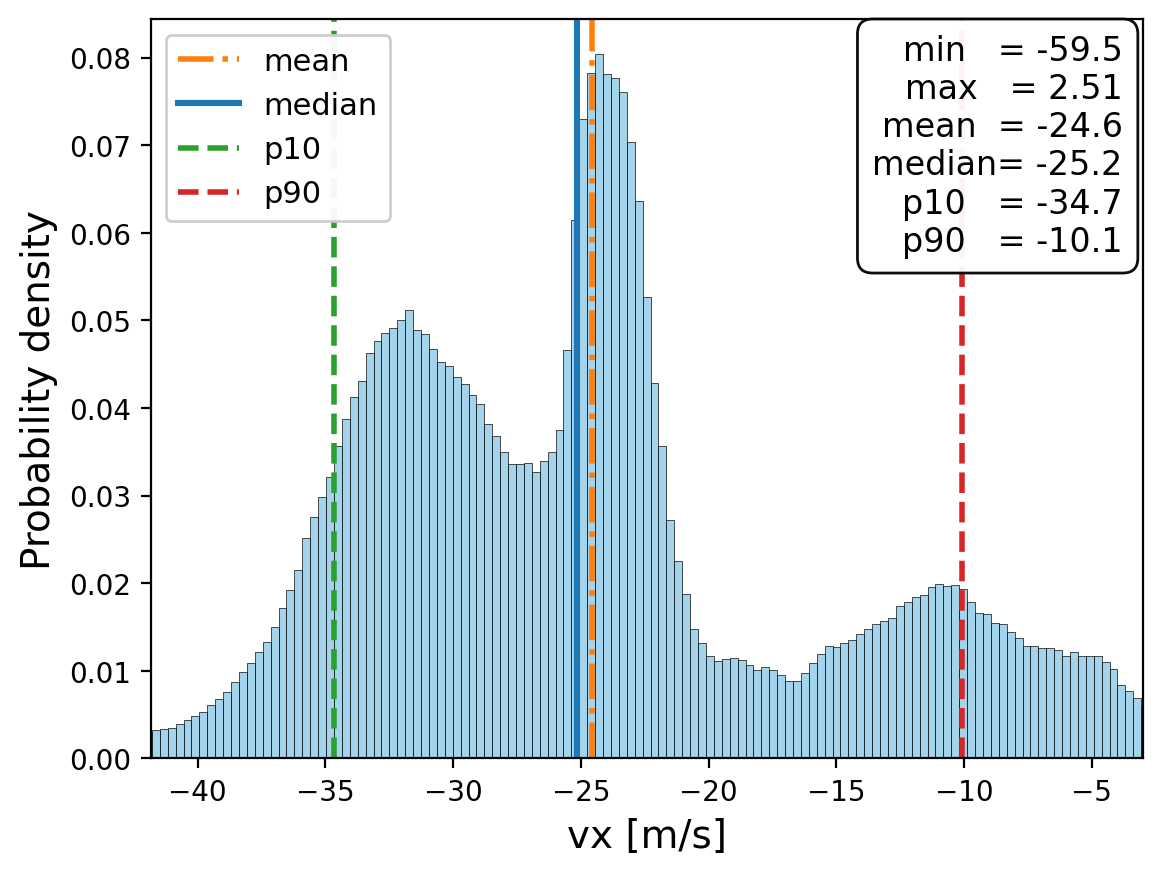
\includegraphics[width=\linewidth]{images/raw_vx__dir1.png}
        \caption{Driving direction 1}
        \label{fig:appendix_raw_vx_dir1}
    \end{subfigure}
    \hfill
    \begin{subfigure}[t]{0.49\textwidth}
        \centering
        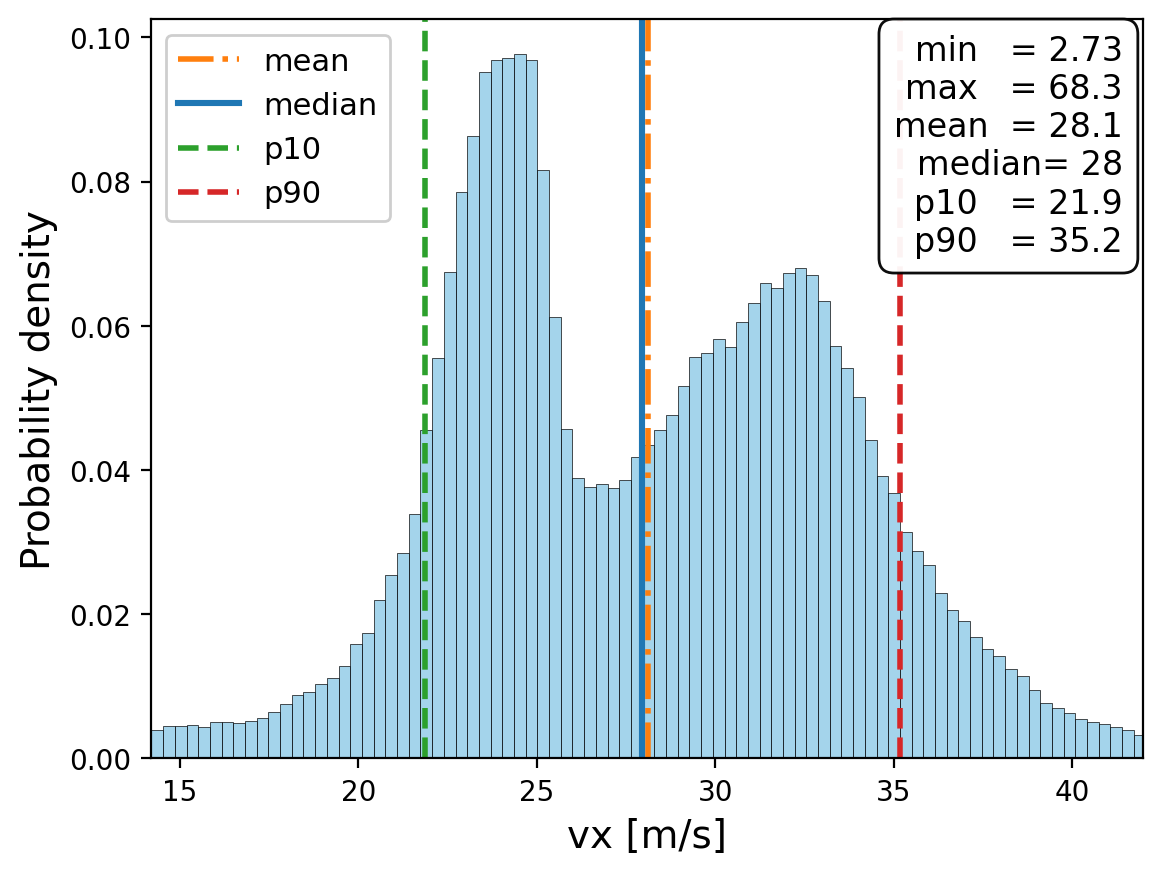
\includegraphics[width=\linewidth]{images/raw_vx__dir2.png}
        \caption{Driving direction 2}
        \label{fig:appendix_raw_vx_dir2}
    \end{subfigure}

    \vspace{0.6em}

    \begin{subfigure}[t]{0.68\textwidth}
        \centering
        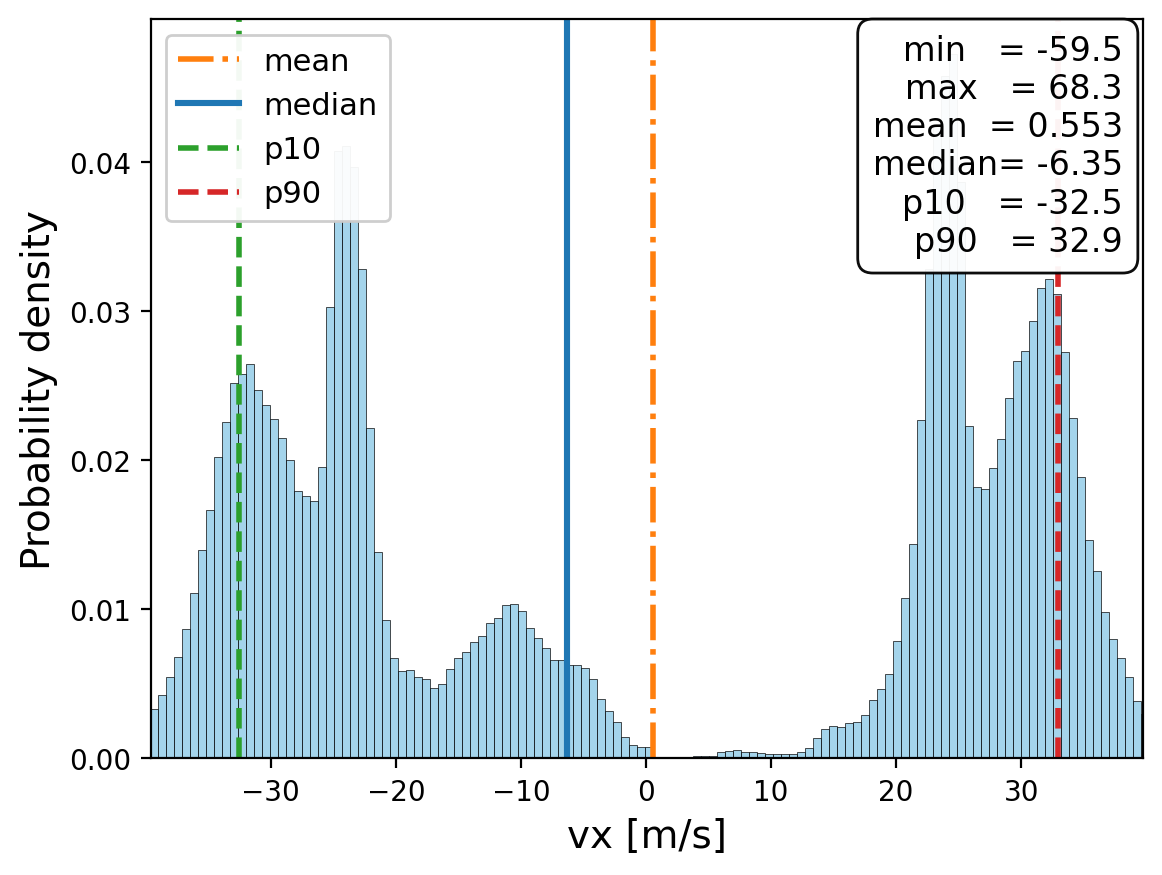
\includegraphics[width=\linewidth]{images/raw_vx__global.png}
        \caption{Combined over both directions.}
        \label{fig:appendix_raw_vx_global}
    \end{subfigure}

    \caption{Direction-wise sign difference in raw longitudinal velocity.}
    \label{fig:appendix_raw_vx_directionwise}
\end{figure}
This appendix illustrates the sign inconsistency in raw highD kinematic signals caused by opposite traffic directions.
For the longitudinal velocity \(v_x\), forward motion appears with opposite signs in the two directions.
As a result, the combined raw distribution is bimodal around zero and cannot be interpreted with a single sign convention.

For completeness, the same raw longitudinal velocity signal is also shown by vehicle class:

\begin{figure}[!htbp]
    \centering

    \begin{subfigure}[t]{0.49\textwidth}
        \centering
        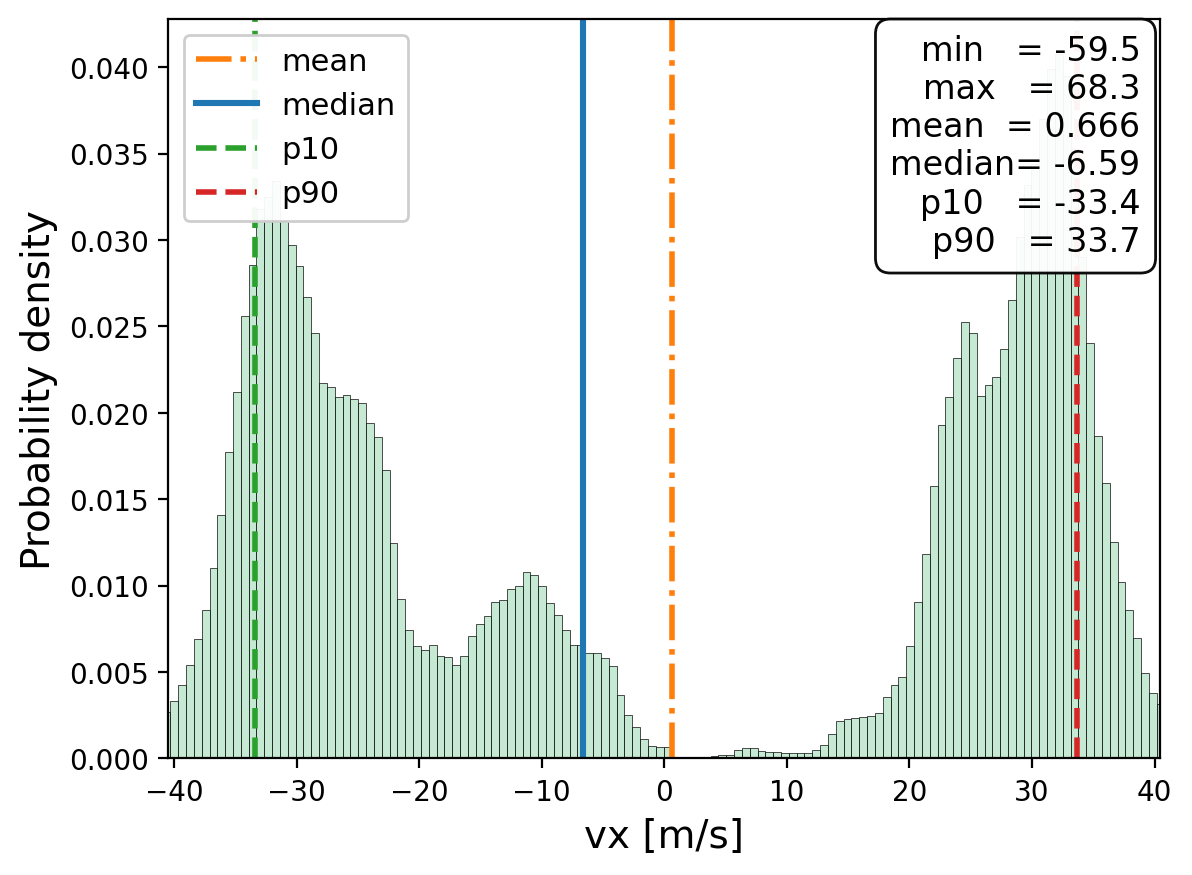
\includegraphics[width=\linewidth]{images/raw_vx__class_car.png}
        \caption{Cars}
        \label{fig:appendix_raw_vx_class_car}
    \end{subfigure}
    \hfill
    \begin{subfigure}[t]{0.49\textwidth}
        \centering
        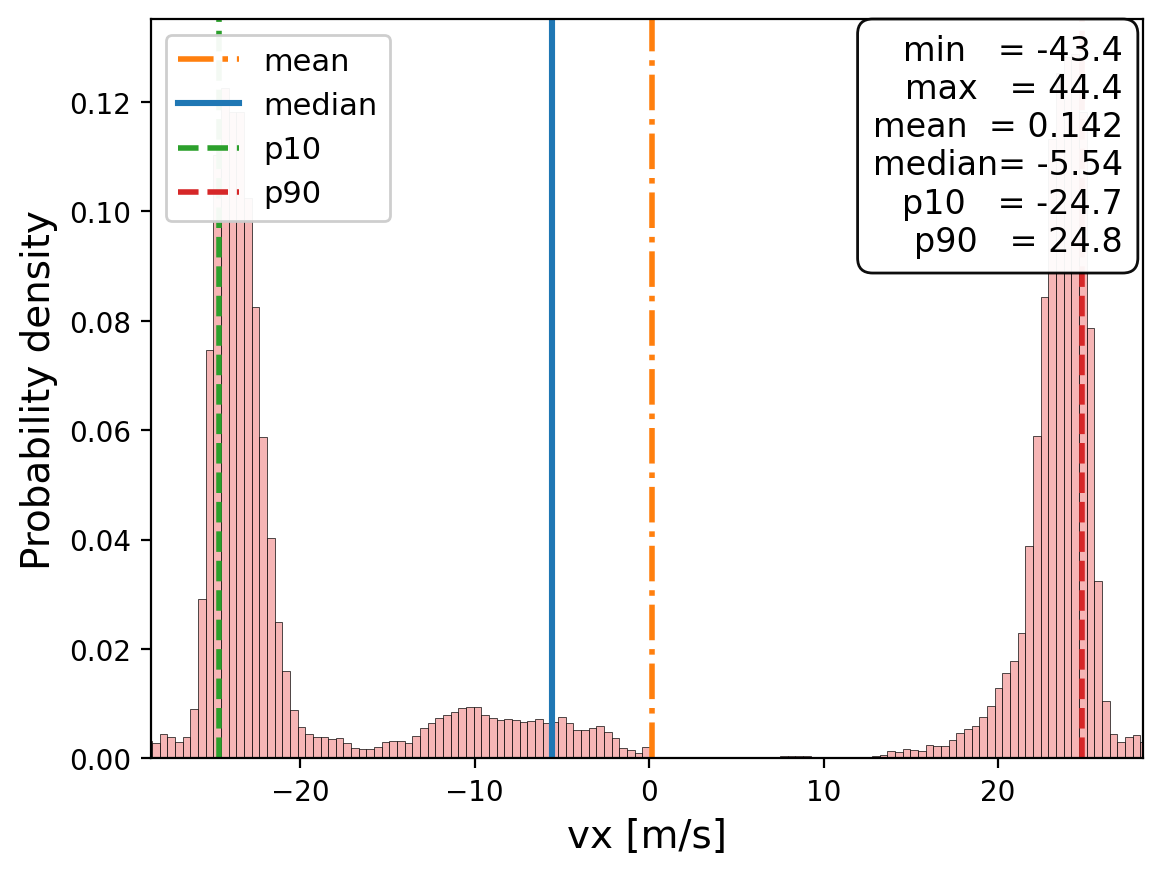
\includegraphics[width=\linewidth]{images/raw_vx__class_truck.png}
        \caption{Trucks}
        \label{fig:appendix_raw_vx_class_truck}
    \end{subfigure}

    \caption{Class-wise raw longitudinal velocity distributions.}
    \label{fig:appendix_raw_vx_classwise}
\end{figure}

